% =============================================================================
% Section 6. The Economic Opportunity Index
% Specification: R/indices/build_economic_opportunity_index_v2.R, R/indices/index_builder_core.R,
% the EO theme builders as called from scripts/10_build_themes.R:
%   R/categories/trade/{trade_core,export_feasibility,trade_concentration}.R
%   R/categories/production/production_depth_momentum.R
%   R/categories/technology_demand/{future_demand,overcapacity_premium}.R
%   R/categories/technological_readiness/technological_readiness.R
%     (+ config/iea_clean_tech_guide_tech_map.yml, stage mapping)
%   R/categories/energy_prices/{energy_prices,lcoe_competitiveness}.R
%   R/categories/investment/investment_momentum.R
%   R/categories/energy_access/energy_access_consumption.R, R/categories/consumption/energy_consumption.R
%   R/categories/foreign_dependency/market_share_manufacturing.R
%   R/categories/economic opportunity/cost_competitiveness.R
% config/weights.yml (economic_opportunity), config/missing_data.yml, config/rankability.yml.
% Results: paper/results/eo.json, scripts/paper/fig_eo.R (final rerun of 2026-10-12);
% fig_eo_transforms.R. Further detail: Online Appendix (sections/oa_eo.tex, oa:eo).
% =============================================================================
\FloatBarrier
\section{The Economic Opportunity Index}\label{sec:eo}\label{sec:economic_opportunity}

The Economic Opportunity pillar $\EO_{its}$ asks how well placed economy $i$ is to capture value
from the expansion of technology $t$ at stage $s$. Its premise comes from economic complexity:
countries diversify into activities close, in capability space, to those they already perform
competitively, and relatedness predicts new comparative advantage
\citep{hidalgo2007product,hausmann2006structural,hausmann2014atlas,hidalgo2009building,hausmann2022implied,hidalgo2021economic,hausmann2007what},
including in low-carbon products \citep{mealy2022economic,growthlab2024greenplexity}. We apply it
at the supply-chain stage, where green industrial policy is now designed
\citep{rodrik2014green,juhasz2024new}, and add market size and growth, cost, technological
maturity and committed capital. A higher score means more opportunity; $\EO_{its}$ is not the
complement of $\ES_{its}$ (Section~\ref{subsec:eo_shared}).

% -----------------------------------------------------------------------------
\subsection{Construction}\label{subsec:eo_aggregation}

Ten categories (Table~\ref{tab:eo_structure}) are combined by the rules of
Section~\ref{sec:normalization} into the available-case weighted mean of
equation~\eqref{eq:pillar}. The weights sum to 30: eight categories carry 3, Technology Demand 4
and Technological Readiness 2. $\Scurve[x]_g$ is the S-curve of equation~\eqref{eq:scurve}
($\gamma=0.5$) within comparison set $g$, by default the pair $(t,s)$. Technological Readiness and
the input-cost component of Cost Competitiveness cover all 33 pairs. Technological Readiness,
Energy Prices and three of the four Technology Demand components are constant within a pair: by
equation~\eqref{eq:affine_constant} they shift a pair's level without reordering its economies.
Appendix~\ref{app:variables} lists every variable; Online Appendix~\ref{oa:eo} gives further
detail.

\begin{table}[tp]
\centering
\begin{threeparttable}
\caption{Structure of the Economic Opportunity pillar}
\label{tab:eo_structure}
\scriptsize
\setlength{\tabcolsep}{3pt}
\begin{tabularx}{\textwidth}{@{}>{\raggedright\arraybackslash}p{1.8cm}
  >{\centering\arraybackslash}p{0.9cm}
  >{\raggedright\arraybackslash}X
  >{\raggedright\arraybackslash}p{2.4cm}
  >{\raggedright\arraybackslash}p{2.3cm}
  >{\raggedright\arraybackslash}p{1.2cm}@{}}
\toprule
Category & Weight (share) & Components (stage: technologies) & Sources & Higher score $=$ & Missing rule\\
\midrule
Trade & 3 (0.10) &
Share of world basket exports; Balassa RCA; basket export value; product-space feasibility;
world export concentration$^{\dagger}$ (Up, Mid: all but Geo, H$_2$) &
Atlas HS92; UN Comtrade &
larger, more specialised exports; closer capabilities; contestable market & avg\\
\addlinespace
Production & 3 (0.10) &
Level, absolute change and a composite of fossil output (Up: Oil, Gas, Coal), uranium mine output
(Up: Nuc), demand-weighted share of world mined mineral supply (Up: Bat, EV, Grid, H$_2$, Sol,
Wind) or power generation (Down: Sol, Wind, Nuc, Coal, Gas, Oil) &
EI Statistical Review; EIA; Red Book; IEA Critical Minerals Dataset &
larger, faster-growing production & avg\\
\addlinespace
Technology Demand & 4 (0.13) &
World supply in 2035 and its growth$^{\dagger}$; regional demand (12 economies) or the EV car
market (Down: EV); US addressable market$^{\dagger}$; manufacturing overcapacity$^{\dagger}$ (Mid:
Bat, Sol, Wind, H$_2$) &
IEA WEO 2025; BNEF NEO 2024; IEA GEVO 2026; BCG; BNEF &
larger, faster-growing market; less overcapacity & avg\\
\addlinespace
Technological Readiness & 2 (0.07) &
TRL Index of the items mapped to the technology and stage: bell-shaped level score and capped
momentum$^{\dagger}$ (all pairs) &
IEA Clean Energy Technology Guide &
readiness nearer TRL 6; faster maturation & avg\\
\addlinespace
Energy Prices & 3 (0.10) &
Commodity price volatility$^{\dagger}$ (Up: all but Geo) & IMF PCPS & lower volatility & avg\\
\addlinespace
Investment & 3 (0.10) &
Investment; three-year momentum; operating and pipeline manufacturing capacity (Up: Bat, EV; Mid:
Bat, EV, Sol, Wind; Down: Bat, EV, Geo, Nuc, Sol, Wind) &
Clean Investment Monitor & more investment and capacity & zero\\
\addlinespace
Energy Access & 3 (0.10) &
Energy supply per capita and its 2020--2025 growth (Down: Coal, Oil, Gas, Sol, Wind, Nuc) &
EI Statistical Review & deeper, growing home market & avg\\
\addlinespace
Foreign Dependency & 3 (0.10) &
Share of world manufacturing capacity incl.\ pipeline (Mid: Bat, Sol, Wind, H$_2$); regional EV
production position (Mid: EV) &
IEA ETP; IEA EV data & larger share of world manufacturing & zero\\
\addlinespace
Cost Competitiveness & 3 (0.10) &
LCOE Index (Down: Bat, Coal, Gas, Sol, Wind); Input Cost Index of wages and capital costs (all
pairs); relative equipment cost (Mid: Bat, Sol, Wind, H$_2$; Down: H$_2$) &
BNEF; ILOSTAT; IMF; IEA & lower costs & none (LCOE); avg\\
\addlinespace
Consumption & 3 (0.10) &
Installed capacity per capita and its growth to 2035 (Down: all but EV, Grid) &
BNEF NEO 2024 & deeper installed base & avg\\
\bottomrule
\end{tabularx}
\begin{tablenotes}[flushleft]\footnotesize
\item \textit{Notes:} Weights from \texttt{config/weights.yml}; shares $w_k/30$ apply where every
category is observed (equation~\eqref{eq:pillar}). Abbreviations as in Table~\ref{tab:es_structure}.
$^{\dagger}$Constant across economies within a pair. Missing rules from
\texttt{config/missing\_data.yml} (Table~\ref{tab:missing_rules}); ``avg'' is the global-average
rule.
\end{tablenotes}
\end{threeparttable}
\end{table}

% -----------------------------------------------------------------------------
\subsection{Categories}\label{subsec:eo_categories}

\paragraph{Trade.}\label{subsec:eo_trade} Trade measures revealed and latent capability to export
the goods of a stage, using the baskets $G_{ts}$ of Section~\ref{subsec:data_crosswalk}; the
upstream baskets give every upstream pair except Geothermal and Green Hydrogen a Trade category. Besides the Atlas
share of world basket exports \citep{growthlab2019trade}, shared with ES, it ranks revealed
comparative advantage \citep{balassa1965trade} from UN Comtrade \citep{uncomtrade},
\begin{equation}\label{eq:eo_rca}
  \RCA_{its}=\frac{E_{its}/T_i}{\sum_{j\in R}E_{jts}\big/\sum_{j\in R}T_j},
\end{equation}
with $E_{its}$ basket and $T_i$ total exports over the reporters $R$; the value of basket exports
$E$; and latent capability, the mean Atlas distance $\delta_{i\eta}$ to the basket's HS four-digit
headings $\mathcal H_{ts}$ \citep{hidalgo2007product},
\begin{equation}\label{eq:eo_feas}
  \mathrm{feas}_{its}=1-\frac{1}{|\mathcal H_{ts}|}\sum_{\eta\in\mathcal H_{ts}}\delta_{i\eta}.
\end{equation}
The fifth component is the world-market concentration term of the ES category, read as
contestability. Then
\begin{equation}\label{eq:eo_trade}
  c_{\mathrm{T},its}=\mean\Big\{\Scurve[\mathrm{ms}]_{ts},\ \Scurve[\RCA]_{ts},\
  \Scurve[E]_{ts},\ \Scurve[\mathrm{feas}]_{ts},\ \Scurve[-\HHI]\Big\}.
\end{equation}
Hong Kong, a re-export hub, is excluded from the Comtrade measures (RCA, export value,
concentration) but keeps its Atlas components, and the concentration term is ranked across the
cells of the eleven headline technologies.

\paragraph{Production.}\label{subsec:eo_production} Production measures the depth of existing
output and its momentum. For oil, gas, coal and uranium upstream and electricity generation
downstream, with output $P_{it,y}$ from the Statistical Review \citep{ei2026statistical} (filled
from EIA where it lists none, Section~\ref{subsec:es_imports}) or the Red Book, and relative and
absolute changes $g^{\mathrm{rel}}$, $g^{\mathrm{abs}}$ over five years,
\begin{equation}\label{eq:eo_prod_energy}
  \mathrm{size}_{its}=\Scurve[P_{\cdot,2025}]_{ts},\qquad
  \mathrm{gabs}_{its}=\Scurve[g^{\mathrm{abs}}]_{ts},\qquad
  O_{its}=\Scurve\Big[\tfrac13\big(\Scurve[P_{\cdot,2025}]+\Scurve[g^{\mathrm{rel}}]
  +\Scurve[g^{\mathrm{abs}}]\big)\Big]_{ts}.
\end{equation}
For the six mineral-intensive technologies upstream, mined supply $S_{im}$ of each mineral in the
IEA base year $y_0$ and in 2035 \citep{iea2026cmdata} enters as a share of base-year world supply
$W_m$, weighted by the technology's demand share $\tilde w_{mt}$:
\begin{equation}\label{eq:eo_prod_mineral}
\begin{gathered}
  s^{y}_{it}=\sum_{m}\tilde w_{mt}\,\frac{S_{im,y}}{W_{m,y_0}},\qquad
  \mathrm{size}_{its}=\Scurve[s^{y_0}]_{ts},\\
  \mathrm{gabs}_{its}=\Scurve[s^{2035}-s^{y_0}]_{ts},\qquad
  O_{its}=\Scurve[2\,\mathrm{size}+\mathrm{gabs}+h_t]_{ts},
\end{gathered}
\end{equation}
so growth is an absolute change in base-year world-share units and $h_t$ is a concentration term
common to the pair. In every cell $c_{\mathrm{P},its}=\tfrac13(\mathrm{size}+\mathrm{gabs}+O)$.

\paragraph{Technology Demand.}\label{subsec:eo_demand} Four sources each contribute one composite.
Two energy outlooks weight growth twice as heavily as size:
\begin{align}
  \mathrm{GD}_{t}&=\Scurve\Big[\tfrac13\big(\Scurve[D_{\cdot,2035}]+2\,\Scurve[D_{\cdot,2035}-D_{\cdot,2024}]\big)\Big],
  \label{eq:eo_weo}\\
  \mathrm{RD}_{it}&=\Scurve\Big[\tfrac13\big(\Scurve[D_{\cdot t,2035}]_t
  +2\,\Scurve\big[D_{\cdot t,2035}/D_{\cdot t,2024}-1\big]_t\big)\Big]_t ,
  \label{eq:eo_bnef}
\end{align}
where $D_{f,y}$ is world supply of fuel $f$ in the World Energy Outlook's Stated Policies Scenario
\citep{iea2025weo}, ranked across seven fuels, and $D_{it,y}$ primary energy consumption in the
twelve economies BloombergNEF models \citep{bnef2024neo}; downstream electric vehicles use the EV
market composite of the Global EV Outlook \citep{iea2026gevo} instead. The third source is BCG's
US serviceable addressable market, one value per pair; the fourth is midstream overcapacity, with
$\rho_t$ the ratio of manufacturing capacity to forecast demand in BloombergNEF's supply-chain data,
\begin{equation}\label{eq:eo_overcap}
  \mathrm{OV}_t=2^{-\rho_t},
\end{equation}
so that capacity equal to demand scores $1/2$ and each further multiple halves the score
(Figure~\ref{fig:eo_transforms}c). Then
\begin{equation}\label{eq:eo_demand}
  c_{\mathrm{TD},its}=\mean\big\{\mathrm{GD}_t,\ \mathrm{RD}_{it},\
  \Scurve[\mathrm{SAM}]_{ts},\ \mathrm{OV}_t\big\}.
\end{equation}

\paragraph{Technological Readiness.}\label{subsec:eo_trl} Opportunity is taken to be greatest
around the demonstration stage, where learning is fast and first-mover positions are open. The
IEA Clean Energy Technology Guide \citep{iea2026cleantechguide} grades technology designs by
readiness level (TRL) for 2020--2025; its post-TRL-9 adoption stages are read as levels 9 to 11.
Ordered rules map each item to a technology and a stage, and a stage without items takes the
technology-wide value. For item $n$ with level $x_n$ and change $\Delta_n$,
\begin{equation}\label{eq:eo_trl_bell}
  b(x)=\begin{cases}
    0, & x\le 2\ \text{or}\ x\ge 11,\\[2pt]
    \cos\!\big(\tfrac{\pi}{2}\,\tfrac{6-x}{4}\big), & 2<x\le 6,\\[4pt]
    \cos\!\big(\tfrac{\pi}{2}\,\tfrac{x-6}{5}\big), & 6<x<11,
  \end{cases}
  \qquad
  \psi(\Delta)=\Big(\frac{\min\{\max\{\Delta,0\},3\}}{3}\Big)^{1/2},
\end{equation}
\begin{equation}\label{eq:eo_trl}
  \mathrm{TRL}_{ts}=\frac{1}{|N_{ts}|}\sum_{n\in N_{ts}}\big[0.7\,b(x_n)+0.3\,\psi(\Delta_n)\big],
\end{equation}
a cardinal index constant within a pair but different across a technology's stages. Of the
Guide's 634 items, 253 map to a headline technology; the index runs from 0.31 (Geothermal
downstream) to 0.72 (Gas downstream).

\begin{figure}[t]
  \centering
  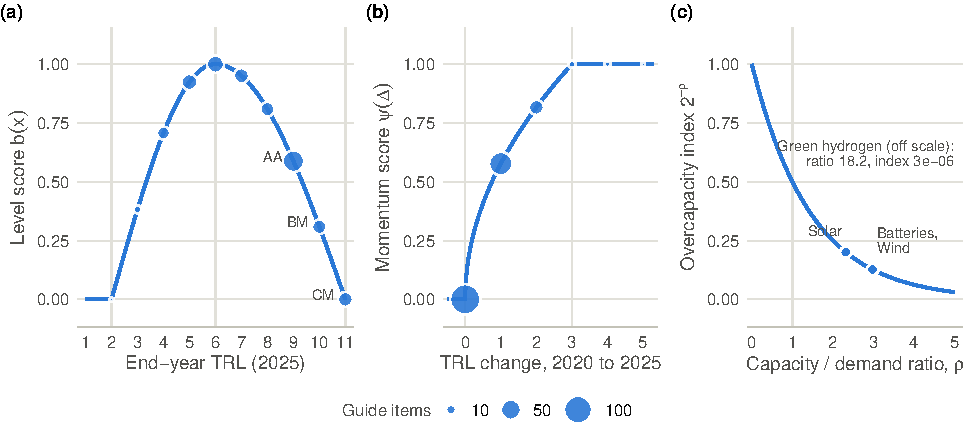
\includegraphics[width=\textwidth]{fig_eo_transforms}
  \caption{The three cardinal transformations of the Economic Opportunity pillar. (a) The level
  score $b(x)$ of equation~\eqref{eq:eo_trl_bell} against the 2025 readiness level; circle area is
  proportional to the number of Guide items mapped to a headline technology at that level (253
  items; TRL 9 to 11 are the Guide's adoption stages: awaiting adoption, building momentum,
  commercial in many markets). (b) The momentum score $\psi(\Delta)$ against the 2020--2025 change,
  capped at three steps. (c) The overcapacity index $2^{-\rho}$ of equation~\eqref{eq:eo_overcap},
  with the four BloombergNEF technologies at their final-build values (green hydrogen, at
  $\rho=18.2$, lies off the scale). Source: the Guide, \texttt{technological\_readiness\_tbl.rds},
  \texttt{overcapacity\_premium\_tbl.rds}; \texttt{scripts/paper/fig\_eo\_transforms.R}.}
  \label{fig:eo_transforms}
\end{figure}

\paragraph{Foreign Dependency: manufacturing position.}\label{subsec:eo_fd} In EO this category
measures the production base from which a country can serve world demand. For batteries, solar,
wind and green hydrogen (the IEA's electrolyser column) it is the S-curve of the share of world
manufacturing capacity including announced projects \citep{iea2024etp}, over the IEA world total
including its residual row; for electric vehicles, four indices of the EV position of the
economy's IEA region, whose five regions partition the world. It carries the zero rule. Every EU
member takes the EU's regional 2035 share (0.15 in wind, 0.11 in batteries, 0.24 in green hydrogen,
0.00 in solar), so EU members are not ranked apart on it.

\paragraph{Cost Competitiveness.}\label{subsec:eo_cost} Three components, one per source. The
levelised cost of electricity of a benchmark plant \citep{bnef2024neo}, today and in 2050,
\begin{equation}\label{eq:eo_lcoe}
  \mathrm{LCOE}_{it}=\tfrac12\Big(\Scurve[-L_{\cdot,y_r}]_t+\Scurve[-L_{\cdot,2050}]_t\Big),
\end{equation}
is defined downstream for five technologies, without imputation. The Input Cost Index prices
labour, $\ell_{is}=\Scurve[\mathrm{wage}]_s$ (ILOSTAT monthly earnings at market exchange rates in
the activity that proxies the stage), and capital, combining the lending rate winsorised and
rescaled to $[0,1]$, $R_i$, with producer-price inflation,
\begin{equation}\label{eq:eo_capital}
  \chi_i=0.6\,R_i+0.4\,\Scurve[\mathrm{infl}]_i ,
\end{equation}
weighted by the stage's factor shares (Table~\ref{tab:eo_factor_shares}),
\begin{equation}\label{eq:eo_ici}
  \mathrm{ICI}_{its}=\frac{\alpha^{L}_{ts}}{\alpha^{L}_{ts}+\alpha^{K}_{ts}}\,\big(1-\ell_{is}\big)
  +\frac{\alpha^{K}_{ts}}{\alpha^{L}_{ts}+\alpha^{K}_{ts}}\,\big(1-\chi_i\big).
\end{equation}
The third is the IEA's regional equipment cost relative to China, $z_{rt}$, and
\begin{equation}\label{eq:eo_cost}
  c_{\mathrm{CC},its}=\mean\big\{\mathrm{LCOE}_{it},\ \mathrm{ICI}_{its},\ 1-\Scurve[z]_{t}\big\}.
\end{equation}

\paragraph{Categories common to both pillars.}\label{subsec:eo_common} Energy Prices, Investment,
Energy Access and Consumption enter EO with the components and index values they have in ES
(Section~\ref{subsec:es_access}). Price volatility is read as investment risk for producers,
investment and pipeline capacity as revealed investor commitment, and per-capita energy use and
installed capacity as the home market.

% -----------------------------------------------------------------------------
\subsection{Shared signals: exposure and capability}\label{subsec:eo_shared}

Table~\ref{tab:shared_signals} lists the raw signals the pillars share, each with the same sign in
both. For export share the readings agree; energy use and installed base also measure the demand
to be secured; and a concentrated world market may signal an entrenched incumbent, as coded, or
unmet demand for an alternative supplier. A shared component induces a positive correlation between
the pillars unrelated to any economic link, while in the Strategic Index (equation~\eqref{eq:si};
variable decomposition of equation~\eqref{eq:var_decomp})
\begin{equation}\label{eq:eo_si_shared}
  \frac{\partial\,\SI_{its}}{\partial x_v}=0.3\,\big(\omega^{\EO}_{k(v),its}\lambda^{\EO}_{v,its}
  -\omega^{\ES}_{k(v),its}\lambda^{\ES}_{v,its}\big),
\end{equation}
where $\omega^{P}_{k,its}$ is the effective weight of the component's category in pillar $P$ and
$\lambda^{P}_{v,its}$ its weight within the category: a shared signal moves the index only as far
as it weighs more in one pillar than in the other. The distinctive information lies in the
non-shared components, which Section~\ref{sec:joint} separates.

\begin{table}[t]
\centering
\begin{threeparttable}
\caption{Raw signals shared by the Energy Security and Economic Opportunity pillars}
\label{tab:shared_signals}
\scriptsize
\setlength{\tabcolsep}{3pt}
\begin{tabularx}{\textwidth}{@{}>{\raggedright\arraybackslash}p{2.0cm}
  >{\raggedright\arraybackslash}p{2.9cm}
  >{\raggedright\arraybackslash}X
  >{\raggedright\arraybackslash}X
  >{\centering\arraybackslash}p{1.3cm}@{}}
\toprule
Category (ES / EO weight) & Shared signal & Reading in ES (security) & Reading in EO (opportunity) & Same index values\\
\midrule
Energy Access (4 / 3) & EI energy supply per capita, level and growth &
availability at the point of use; equally the demand to be secured &
depth and growth of the home market & yes\\
\addlinespace
Consumption (5 / 3) & BNEF installed capacity per capita, level and growth &
depth of the installed base & home market for equipment and services & yes\\
\addlinespace
Investment (3 / 3) & CIM investment, momentum and capacity &
future domestic supply & revealed investor commitment & yes\\
\addlinespace
Energy Prices (2 / 3) & IMF commodity price volatility & price risk for users &
investment risk for producers & yes (cell constant)\\
\addlinespace
Trade (4 / 3) & Atlas export market share; world export concentration &
a supplier rather than a dependent; few suppliers is a risk &
revealed capability; a concentrated market is less contestable & two of three / five\\
\addlinespace
Foreign Dependency (6 / 3) & IEA manufacturing-capacity share; IEA EV regional position &
domestic capacity reduces dependence & production base to serve world demand &
yes; different missing rules\\
\addlinespace
Production (6 / 3) & mined output of the technology's minerals &
domestic supply (demand-weighted, zero-anchored) & demand-weighted share of world supply and its
projected change & no\\
\bottomrule
\end{tabularx}
\begin{tablenotes}[flushleft]\footnotesize
\item \textit{Notes:} Nominal category weights of \texttt{config/weights.yml} (ES out of 42, EO
out of 30). ``Same index values'': the component enters both pillars as the same theme-level
value; imputed values can differ where the missing-data rules or country grids differ.
\end{tablenotes}
\end{threeparttable}
\end{table}

% -----------------------------------------------------------------------------
\subsection{Results}\label{subsec:eo_results}

\paragraph{Coverage and rankability.} The pillar scores 7{,}131 cells of the eleven headline
technologies for 219 economies (195 sovereign, 24 territories) in all 33 pairs, none constant.
Twenty-four cells are fully imputed (the Isle of Man 14, Puerto Rico 8, Liechtenstein 2); the mean
imputed weight share is 0.43 (0.41, 0.44 and 0.43 by stage). The rankability rule admits 4{,}301
cells for 178 economies, from 40 in Green Hydrogen midstream to 175 in Nuclear upstream. The
excluded cells would mostly have ranked low: they hold only three of the 330 top-ten places
computed over all scored economies, and no first place.

\paragraph{Distribution and variance.} The median rankable cell scores 0.500 upstream, 0.501
midstream and 0.488 downstream (interquartile ranges 0.434--0.542, 0.427--0.561 and 0.427--0.551;
Figure~\ref{fig:eo_distribution}). Differences between technologies dominate: pair medians range
from 0.367 to 0.585 upstream and from 0.351 to 0.579 midstream, against a mean within-pair
interquartile range of 0.037 and 0.082. The clean-technology midstream pairs sit lowest because
they carry Foreign Dependency and Investment under the zero rule. Technology-stage fixed effects
explain 57.9 per cent of the variance, country effects alone 17.7 per cent and both 77.2 per cent
(45.8 per cent of the within-pair variance; ES: 44.4 and 27.8 per cent). Cross-pair comparisons of
EO levels, as in the Strategic Index, compare mostly pair effects.

\paragraph{Drivers.} In the level (Figure~\ref{fig:eo_contrib}), Cost Competitiveness has the
largest share at every stage (21.9, 29.2 and 27.5 per cent), followed by Technology Demand. In the
within-pair variance, Technological Readiness and Energy Prices contribute nothing and Technology
Demand 2 to 6 per cent; the categories that order economies are Cost Competitiveness (39.2, 37.6 and
21.7 per cent by stage), Trade and Production upstream, Trade and Foreign Dependency midstream, and
Consumption and Investment downstream. Six technology-level constants carry 38.9 per cent of the
average rankable cell's effective weight (46.3, 40.4 and 27.9 per cent by stage), imputed country
inputs 17.5 per cent and observed country-specific information 43.6 per cent
(Table~\ref{tab:eo_weight_split}): the pillar's cross-country content is thinnest upstream.

% Written by scripts/paper/fig_eo.R from the objects saved in paper/results/eo.json (keys: input_weights, coverage).
\begin{table}[tbp]
\centering
\begin{threeparttable}
\caption{Effective weight of the Economic Opportunity pillar by type of input}
\label{tab:eo_weight_split}
\small
\begin{tabular}{@{}l S[table-format=2.1] S[table-format=2.1] S[table-format=2.1] S[table-format=2.1]@{}}
\toprule
 & \multicolumn{3}{c}{Mean effective weight (per cent)} & {Constants' share}\\
\cmidrule(lr){2-4}
 & {Technology-level} & {Imputed,} & {Observed,} & {of the level}\\
 & {constants} & {country-varying} & {country-varying} & {(per cent)}\\
\midrule
Upstream & 46.3 & 19.7 & 33.9 & 44.0\\
Midstream & 40.4 & 14.6 & 45.0 & 40.2\\
Downstream & 27.9 & 17.4 & 54.7 & 30.4\\
\addlinespace
All rankable cells & 38.9 & 17.5 & 43.6 & 38.7\\
All scored cells & 37.7 & 30.1 & 32.3 & 39.5\\
\bottomrule
\end{tabular}
\begin{tablenotes}[flushleft]\footnotesize
\item \textit{Notes:} The effective weight of variable $v$ in cell $(i,t,s)$ is the renormalised category weight times the variable's weight within its category, $\omega_{kits}\lambda_{vkits}$ (equation~\eqref{eq:var_decomp}); it sums to one in every cell. Technology-level constants are the variables whose value has zero range across all scored economies of the pair: the TRL Index (one value per technology and stage), the WEO global-demand composite, the BCG addressable market, the overcapacity index, the world-market concentration term of Trade and commodity-price volatility. Imputed components are those filled by a missing-data rule (global average or zero) for the economy in question. The first three columns sum to 100 within a row, up to rounding. The last column is the mean share of $\EO_{its}$ contributed by the constants. Rows by stage and ``All rankable cells'': means over the 1{,}681 upstream, 1{,}307 midstream and 1{,}313 downstream rankable cells of the eleven headline technologies (a sovereign economy with at most half of the cell's weight imputed); ``All scored cells'': means over all 7{,}131 scored cells. Source: \texttt{economic\_opportunity\_variable\_contributions} in \texttt{data/processed/outputs/index\_outputs.rds}; \texttt{scripts/paper/fig\_eo.R}.
\end{tablenotes}
\end{threeparttable}
\end{table}


\paragraph{Leaders.} China leads 22 of the 33 pairs, the United States five, Chad three, and
Canada, Indonesia and Saudi Arabia one each (Table~\ref{tab:eo_leaders}); emerging economies,
mostly China, hold 26 first places and 46.4 per cent of the top-ten places. Chad's three pairs
(Geothermal upstream and midstream, Electric Grid downstream) are those in which only Cost
Competitiveness varies, and its leads rest on a recorded lending rate at the floor of the rescaled
rate: artefacts, not evidence of opportunity. The median leader's margin is 0.043; China's in
Green Hydrogen, Wind, Solar and Batteries midstream are 0.14 to 0.20. In Batteries midstream
(Figure~\ref{fig:eo_top}) China's lead over the United States comes from its manufacturing share
and costs; in Solar midstream five Southeast Asian partners take five of the top ten places.

\paragraph{The coalition.} Over their rankable cells the 31 core members have a mean within-pair
percentile of 0.66, the 26 partners 0.49, other economies 0.44 and China 0.96
(Figure~\ref{fig:eo_heatmap}). The core is strongest midstream (0.73). The best-placed member is
first in 8 pairs and in the top three of 30; in 14 pairs it is a partner, and Indonesia ranks
second behind China in five upstream mineral pairs. Both ends of the member ranking are partly
construction: four members (T\"urkiye, Brazil, Argentina, Ghana) record nominal lending rates at the
winsorisation ceiling, which depresses every pair, and the BNEF regional composite ranks some
modelled economies below unmodelled ones (Online Appendix~\ref{oa:eo}).

% Written by scripts/paper/fig_eo.R from the objects saved in paper/results/eo.json (key: leaders).
\begin{table}[tbp]
\centering
\begin{threeparttable}
\caption{Leading economies in each technology-stage pair of the Economic Opportunity pillar (rankable cells)}
\label{tab:eo_leaders}
\footnotesize
\begin{tabular}{@{}lrlllcrr@{}}
\toprule
Technology & $n$ & First & Second & Third & Best member (rank) & USA & CHN \\
\midrule
\multicolumn{8}{@{}l}{\textit{Upstream}}\\
Batteries & 120 & CHN 0.65 & IDN 0.59 & AUS 0.57 & IDN (2) & 7 & 1 \\
Coal & 157 & IDN 0.52 & CHN 0.51 & IND 0.48 & IDN (1) & 7 & 2 \\
Electric Grid & 163 & CHN 0.71 & CHL 0.65 & RUS 0.65 & CHL (2) & 27 & 1 \\
Electric Vehicles & 153 & CHN 0.68 & IDN 0.62 & AUS 0.57 & IDN (2) & 4 & 1 \\
Gas & 165 & USA 0.61 & CHN 0.60 & CAN 0.57 & USA (1) & 1 & 2 \\
Geothermal & 141 & TCD 0.48 & CMR 0.48 & COG 0.48 & PRT (4) & 68 & 6 \\
Green Hydrogen & 146 & CHN 0.62 & IDN 0.62 & ZMB 0.57 & IDN (2) & 62 & 1 \\
Nuclear & 175 & CAN 0.65 & CHN 0.62 & KAZ 0.62 & CAN (1) & 6 & 2 \\
Oil & 166 & USA 0.66 & CHN 0.64 & CAN 0.64 & USA (1) & 1 & 2 \\
Solar & 153 & CHN 0.70 & IDN 0.66 & THA 0.61 & IDN (2) & 23 & 1 \\
Wind & 142 & CHN 0.70 & IDN 0.59 & USA 0.58 & IDN (2) & 3 & 1 \\
\addlinespace
\multicolumn{8}{@{}l}{\textit{Midstream}}\\
Batteries & 54 & CHN 0.77 & USA 0.63 & HUN 0.55 & USA (2) & 2 & 1 \\
Coal & 155 & CHN 0.59 & POL 0.57 & IDN 0.56 & POL (2) & 14 & 1 \\
Electric Grid & 162 & CHN 0.68 & THA 0.64 & POL 0.62 & THA (2) & 14 & 1 \\
Electric Vehicles & 145 & CHN 0.74 & ESP 0.64 & USA 0.63 & ESP (2) & 3 & 1 \\
Gas & 156 & CHN 0.71 & IND 0.67 & ITA 0.65 & IND (2) & 5 & 1 \\
Geothermal & 141 & TCD 0.64 & CMR 0.64 & COG 0.64 & PRT (4) & 58 & 5 \\
Green Hydrogen & 40 & CHN 0.71 & DEU 0.50 & USA 0.50 & DEU (2) & 3 & 1 \\
Nuclear & 154 & CHN 0.65 & FRA 0.65 & IND 0.62 & FRA (2) & 21 & 1 \\
Oil & 156 & CHN 0.72 & AUT 0.67 & ITA 0.66 & AUT (2) & 11 & 1 \\
Solar & 79 & CHN 0.79 & IND 0.64 & USA 0.63 & IND (2) & 3 & 1 \\
Wind & 65 & CHN 0.74 & POL 0.54 & IND 0.52 & POL (2) & 4 & 1 \\
\addlinespace
\multicolumn{8}{@{}l}{\textit{Downstream}}\\
Batteries & 140 & CHN 0.75 & USA 0.67 & ITA 0.63 & USA (2) & 2 & 1 \\
Coal & 104 & CHN 0.68 & IDN 0.66 & IND 0.66 & IDN (2) & 15 & 1 \\
Electric Grid & 141 & TCD 0.68 & CMR 0.68 & TGO 0.67 & THA (11) & 109 & 20 \\
Electric Vehicles & 105 & CHN 0.75 & VNM 0.73 & THA 0.70 & VNM (2) & 29 & 1 \\
Gas & 104 & USA 0.72 & SAU 0.71 & CHN 0.68 & USA (1) & 1 & 3 \\
Geothermal & 128 & USA 0.61 & IDN 0.46 & PRT 0.42 & USA (1) & 1 & 16 \\
Green Hydrogen & 158 & USA 0.65 & DEU 0.60 & THA 0.60 & USA (1) & 1 & 4 \\
Nuclear & 86 & CHN 0.72 & FRA 0.67 & JPN 0.64 & FRA (2) & 15 & 1 \\
Oil & 104 & SAU 0.71 & IRN 0.69 & QAT 0.68 & SAU (1) & 8 & 98 \\
Solar & 148 & CHN 0.75 & USA 0.67 & IND 0.67 & USA (2) & 2 & 1 \\
Wind & 95 & CHN 0.70 & USA 0.61 & CAN 0.60 & USA (2) & 2 & 1 \\
\bottomrule
\end{tabular}
\begin{tablenotes}[flushleft]\footnotesize
\item \textit{Notes:} $\EO_{its}$ for the eleven headline technologies. Only rankable cells enter: a sovereign economy with at most half of the cell's index weight imputed (\texttt{config/rankability.yml}). Economies are identified by ISO3 code and followed by their score; $n$ is the number of rankable economies in the pair (40 to 175). ``Best member'' is the highest-ranked of the 57 coalition members (31 core, 26 partners), with its rank in parentheses; the USA and CHN columns give the ranks of the United States and China. A rank is one plus the number of rankable economies with a strictly higher score. All 33 pairs are scored and none is constant across economies. In geothermal upstream and midstream and electric-grid downstream, Cost Competitiveness is the only category that varies across economies. Codes: AUS Australia, AUT Austria, CAN Canada, CHL Chile, CMR Cameroon, COG Congo, DEU Germany, ESP Spain, FRA France, HUN Hungary, IDN Indonesia, IND India, IRN Iran, ITA Italy, JPN Japan, KAZ Kazakhstan, POL Poland, PRT Portugal, QAT Qatar, RUS Russia, SAU Saudi Arabia, TCD Chad, TGO Togo, THA Thailand, VNM Viet Nam, ZMB Zambia, USA United States, CHN China. Source: \texttt{economic\_opportunity\_index} in \texttt{data/processed/outputs/index\_outputs.rds}; \texttt{scripts/paper/fig\_eo.R}.
\end{tablenotes}
\end{threeparttable}
\end{table}


\begin{figure}[tbp]
  \centering
  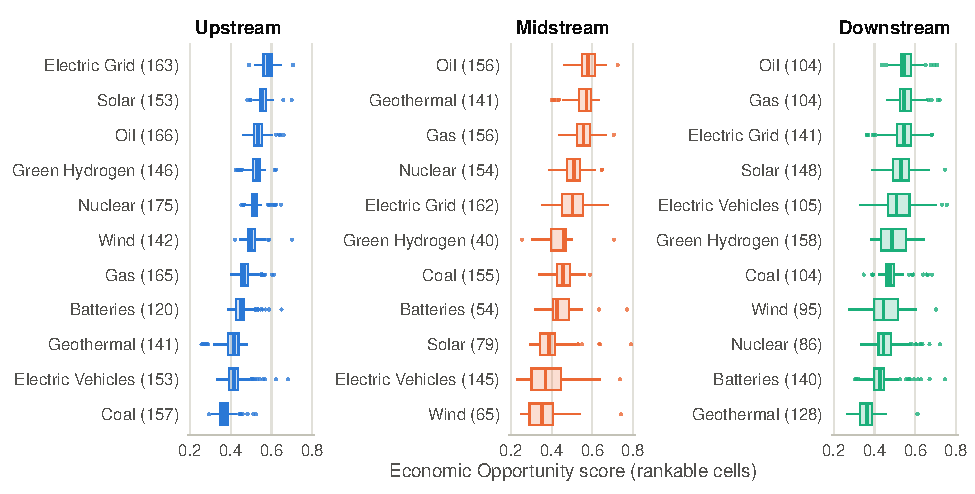
\includegraphics[width=\textwidth]{eo_distribution}
  \caption{Economic Opportunity by technology and stage over the rankable economies of each pair
  (number in parentheses, 40 to 175; sovereign economy with at most half of the index weight
  imputed). Boxes show the median and interquartile range, whiskers 1.5 interquartile ranges.
  Sample: 4{,}301 rankable of 7{,}131 scored cells; all 33 pairs have status \emph{ok}. Source:
  \texttt{economic\_opportunity\_index} in \texttt{index\_outputs.rds};
  \texttt{scripts/paper/fig\_eo.R}.}
  \label{fig:eo_distribution}
\end{figure}

\begin{figure}[tbp]
  \centering
  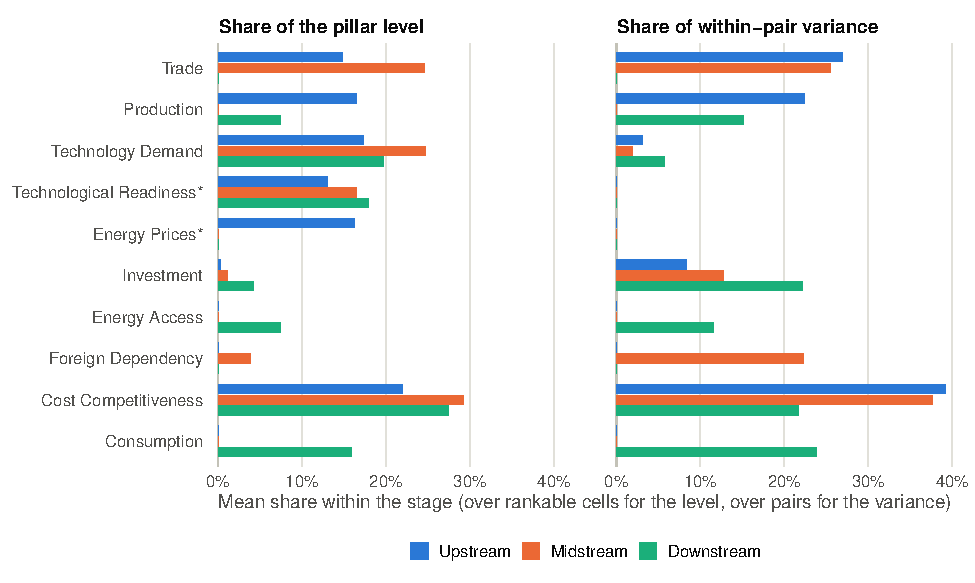
\includegraphics[width=\textwidth]{eo_contrib}
  \caption{Composition of Economic Opportunity by stage. Left: mean share of each category in the
  level, $\omega_{kits}c_{kits}/\EO_{its}$ (equation~\eqref{eq:cat_decomp}). Right: mean share in
  the within-pair variance, $\mathrm{cov}(\omega_{kits}c_{kits},\EO_{its})/\mathrm{var}(\EO_{its})$.
  Starred categories (Technological Readiness, Energy Prices) are constant within every pair;
  Technology Demand is constant except for its BNEF regional and EV-market composites. Sample:
  4{,}301 rankable cells. Source: category contributions in \texttt{index\_outputs.rds};
  \texttt{scripts/paper/fig\_eo.R}.}
  \label{fig:eo_contrib}
\end{figure}

\begin{figure}[tbp]
  \centering
  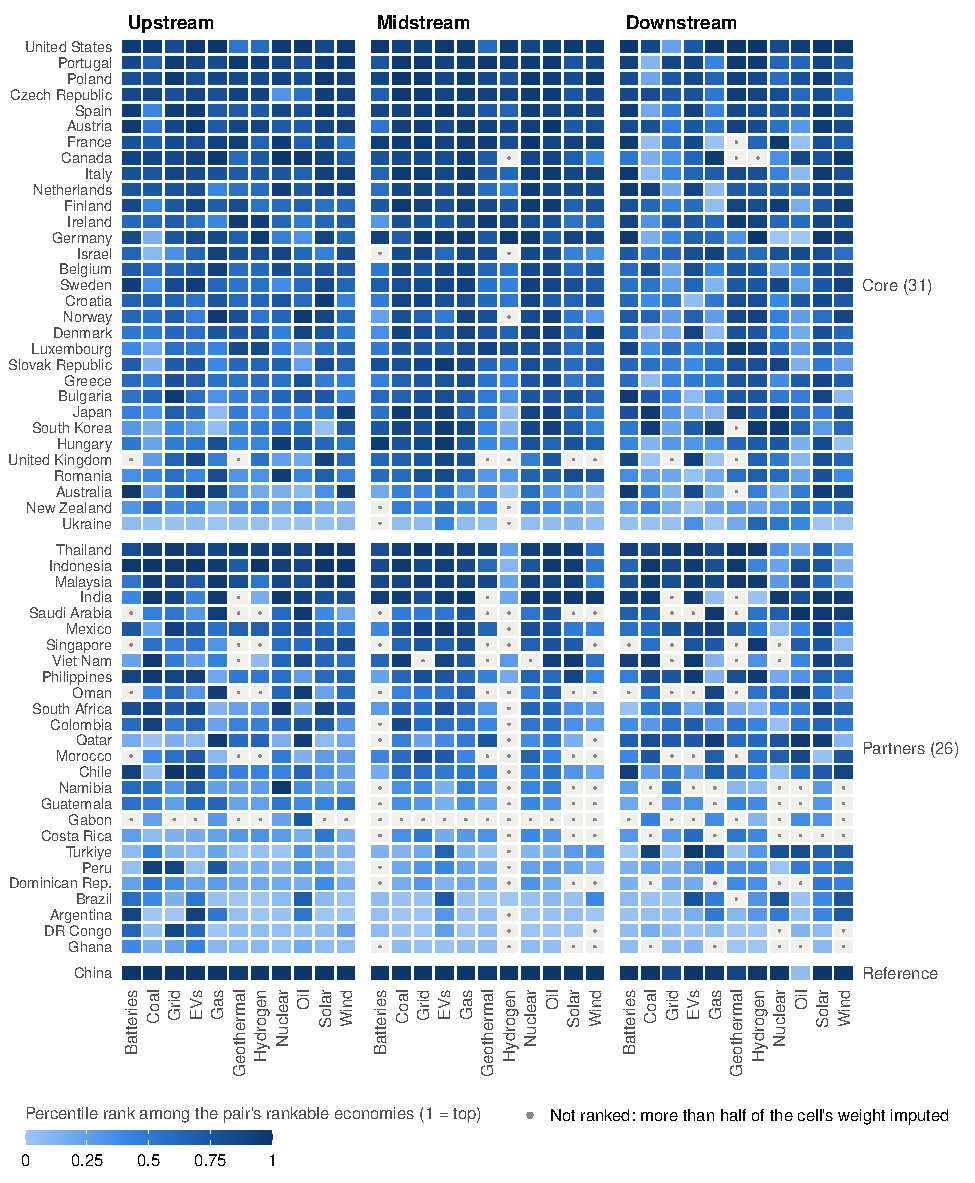
\includegraphics[width=\textwidth]{eo_heatmap}
  \caption{Within-pair percentile rank of $\EO_{its}$ (equation~\eqref{eq:pct_rank}) of the 31
  core members, the 26 partners (Section~\ref{sec:coalition}) and China, by pair. Ranks rather than
  levels are shown because pair effects account for 58 per cent of the variance of the level. Gray
  cells with a dot are scored but not rankable (more than half of the weight imputed). Source:
  \texttt{economic\_opportunity\_index}, \texttt{coalition\_members}; \texttt{scripts/paper/fig\_eo.R}.}
  \label{fig:eo_heatmap}
\end{figure}

\begin{figure}[tbp]
  \centering
  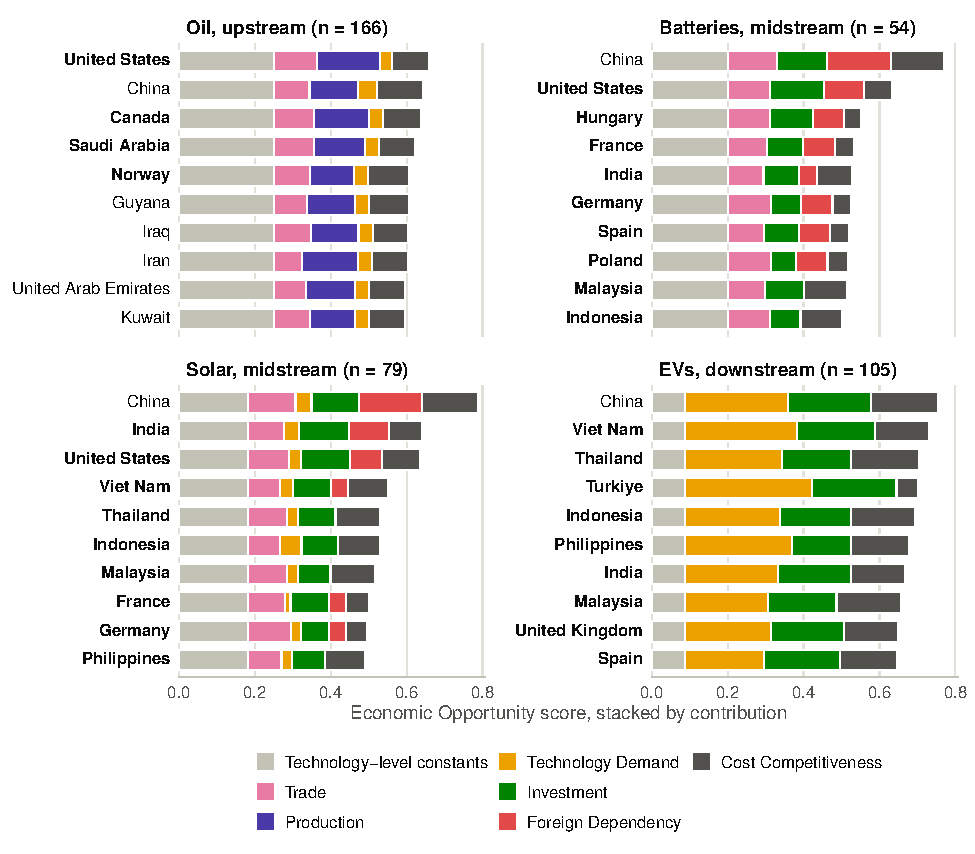
\includegraphics[width=\textwidth]{eo_top}
  \caption{The ten highest-scoring rankable economies in Oil upstream ($n=166$), Batteries
  midstream (54), Solar midstream (79) and EV downstream (105), stacked by the variable
  decomposition of equation~\eqref{eq:var_decomp}; colour identifies the category. The gray segment
  sums the technology-level constants (0.250, 0.202, 0.181 and 0.088), the same for every economy
  in a pair. Coalition members in bold. Source: \texttt{economic\_opportunity\_index} and its
  variable contributions; \texttt{scripts/paper/fig\_eo.R}.}
  \label{fig:eo_top}
\end{figure}

\FloatBarrier
